\documentclass[12pt,a4paper]{report}
\usepackage[utf8]{inputenc}
\usepackage[spanish]{babel}
\usepackage{amsmath}
\usepackage{amsfonts}
\usepackage{amssymb}
\usepackage{graphicx}
\usepackage[left=2cm,right=2cm,top=2cm,bottom=2cm]{geometry}
\author{Oscar Cruz Cervantes}
\title{2_3_Explicar_los_arreglos_y_parametros_de_los_Amplificadores_Clase_B}

\begin{document}

\begin{center}
EV. 2.3\\

Oscar Cruz Cervantes 18311638\\
Sistemas electronicos de interfaz\\
Ing. Mecatronica 4ºB\\


\includegraphics[scale=1.5]{01.png}\\
Explicar los arreglos y parametros de los Amplificadores Clase B
\end{center}
\newpage
\section{Amplificadores clase B}
\begin{center}
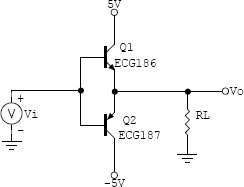
\includegraphics[scale=1]{01.jpg}\\
En esta operaciòn, se usa un transistor para amplificar el ciclo positivo de la señal de entrada, mientras un segundo dispositivo se preocupa del ciclo negativo. La configuracion se conoce como push-pull.
\end{center}


\begin{center}
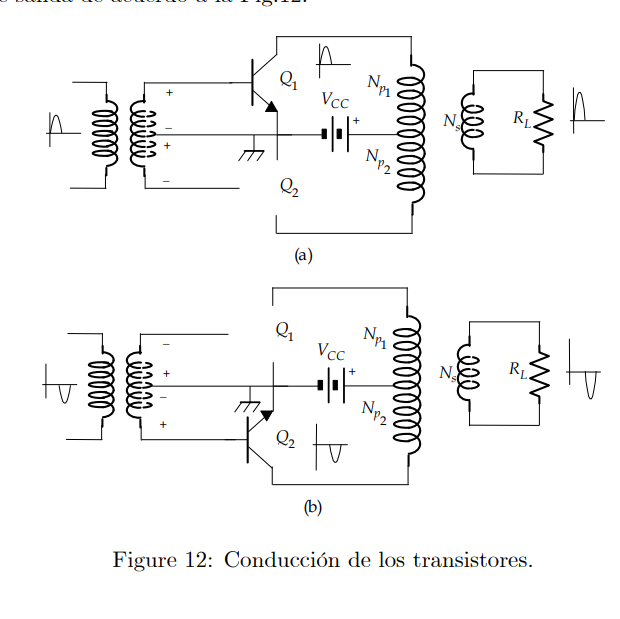
\includegraphics[scale=0.5]{02.png}
\end{center}
En este tipo de aplificador se utilizan dos dispositivos, estos se pone a manera de espejo pues los amplificadores clase b solo pueden conducir un semi-ciclo ya sea el positivo o el negativo segun su acomodo. Como podemos observar en la imagen anterior cuando en voltaje es positivo un transistor conduce y el otro esta en corte y cuando el voltaje es negativo el otro transistor conduce y el primero se encuentra en corte.\\
\cite{amplificadores}
\bibliographystyle{apalike} 
\bibliography{biblio}

\end{document}